\chapter{Sonar Modelbus Plugin} \label{sec:sonar_modelbus_plungin}

\section{Modelbus} \label{sec:modelbus}
\subsection{Scenario}

Imagine, you are in a software developement process. You and your team partners use different developement tools and a lot of artifacts are produced by different team members. In such a case, the artifacts may be inconsitent and a developer needs to make updates and changes by hand to keep them consistent. A tool which would automate this process and do more, is ModelBus.

\subsection{What is ModelBus?}

It is a model-driven open source framework for the integration of development tools during a MDE process. It keeps the artifacts of the development process consistent. It offers a communication between tools with the help of adapters: the tools are connected to the bus via adapters and can offer their services to other tools connected to the bus.

\subsection{Goals}
\begin{itemize}
\item Data Integration: Tools can share (data) models
\item Control Integration: Tools connected to the bus can use the service of other connected tools
\item Process Integration: Several tools are used together in the development and are highly supported
\item Support: Support of distributed MDE development
\item Architecture: Based on SOA
\end{itemize}

\subsection{Architecture}
\begin{itemize}
\item based on SOA
\item central bus-like communication structure
\item number of core services
\item a couple of model management tools
\item different tools can be added to the bus via adapters
\item if a tool is connected, it is handled as a service for other tools
\item orchestration: a lot of tools (with their service) and automation are connected together to a complex system
\end{itemize}

\begin{figure}
	\centering
		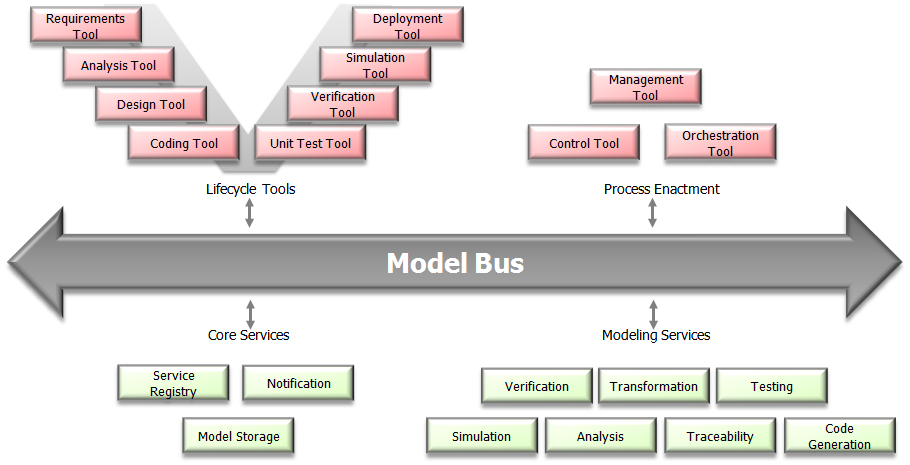
\includegraphics[width=\textwidth]{modelbus_1}
	\caption{Modelbus tools and services}
	\label{fig:sonarrunning}
\end{figure}

\begin{figure}
	\centering
		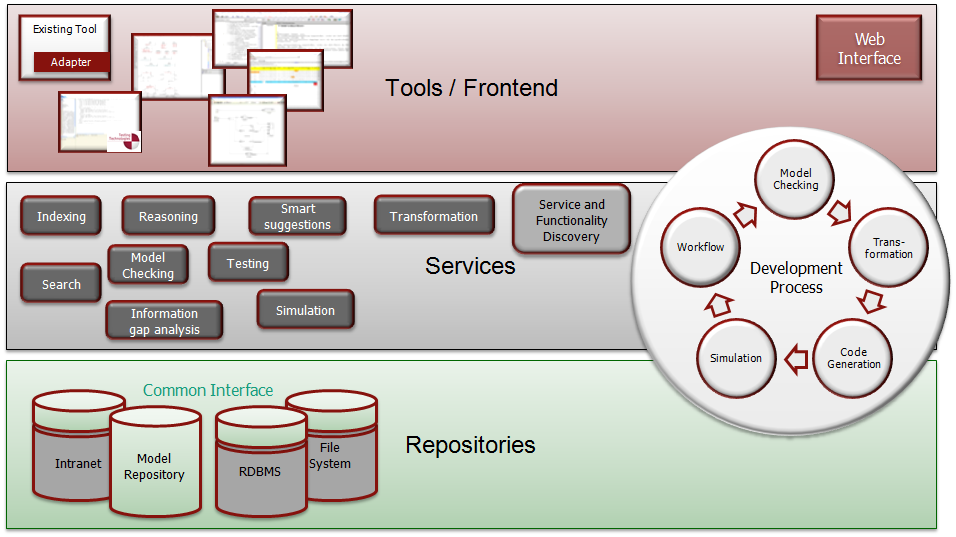
\includegraphics[width=\textwidth]{modelbus_2}
	\caption{Developement process and layers}
	\label{fig:sonarrunning}
\end{figure}

\subsection{Features}

\subsubsection{Automation of development tasks}

\begin{itemize}
\item define tasks as modeling services
\item orchestrate defined tasks with other modelling services
\item orchestrations can be run automatically (by user or other orchestrations)
\end{itemize}

\subsubsection{Inbuilt and transparent model management}

\begin{itemize}
\item problem: development produces artifacts and developer don't want to care about where they came from and how they have to be imported
\item artifacts are acceessed to the rigth model by each connected tool on the ModelBus bus
\end{itemize}

\subsubsection{Support of large and complex models}

\begin{itemize}
\item models often have complex structure
\item model A imports parts if model B and B references package C and ...
\item thus, a lof ot developers work on the models concurrently
\item solution: versioning of (complex) models and model fragments in the model repository
\item core service notification: notification system, which informs about changes to a model
\end{itemize}

\subsubsection{Distributed and heterogeneous}

\begin{itemize}
\item normally, if a tool is updated, different artifacts may be non-compatible together
\item this may happen frequently in larger development teams
\item but this would be crucial, espepcially for model operations tools (for example tools, which transform models)
\item solution: via the adapters, models from the tools are translated into a ModelBus known format
\item distribution of models is therefore realized
\item data models stay consistent, even when tools are updated
\end{itemize}

\subsubsection{Built on industry standards}

\begin{itemize}
\item Transportation: HTTP, HTTPS, XMPP, CXF, JMS, SOAP
\item Core services: Distributed OSGi, SVN, EMF
\item  ...
\end{itemize}

\subsection{Adapters for tools}

\begin{itemize}
\item Doors
\item Eclipse Papyrus
\item Enterprise Architect
\item Eclipse TeamProvider
\item Office
\item Rational Software Architect
\item Rhapsody
\item Simulink
\end{itemize}

\section{Metrino} \label{sec:metrino}

\subsection{Short facts}

\begin{itemize}

\item Validating models by information quantity and quality
\item Uses OCL (Object Constraint Language) and SMM (Software Metrics Metamodel)
\item Can be used as stand-alone tool or as ModelBus add-on with additional service features
\item Works as a set of support tools in four conceptual phases
\item Check of these selectable guidelines result in validation, warnings and/or errors
\item Handles UML models, any Domain Specific Modeling Language (DSL) based on MOF
\item Manage and compute generated or user-defined, domain specific measures
\item Already includes a set of metrics in the current version
\item Supports customizable report generation to different formats
\item Supports visualization of computational results, e.g. graphs
\item Installation by Eclipse update-site through ModelBus website: http://www.modelbus.org/metrino/downloads/current/site.xml
\end{itemize}

\subsection{Four phases}

\begin{figure}[h]
	\centering
		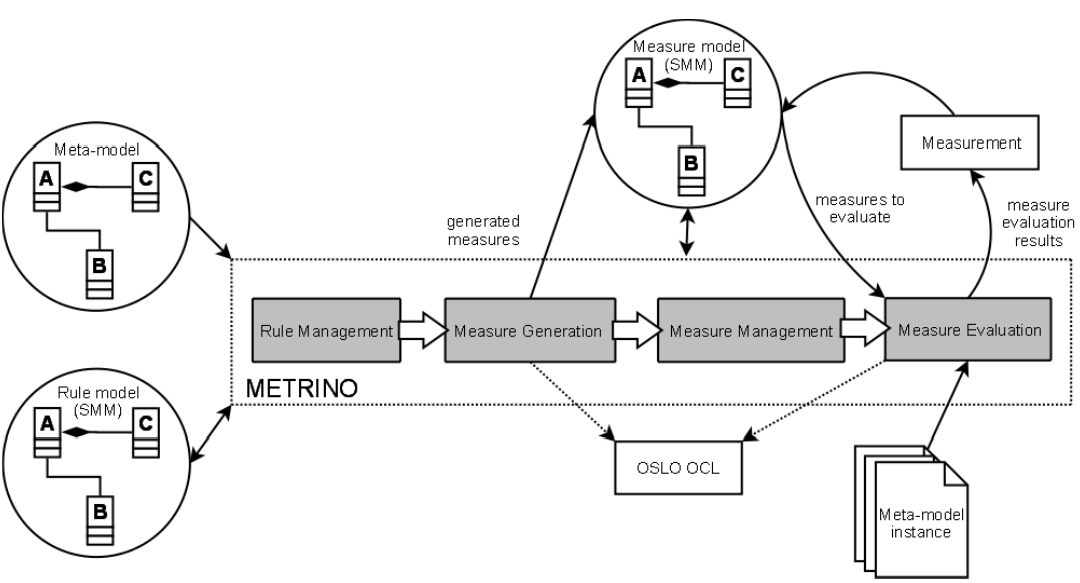
\includegraphics[width=\textwidth]{metrino_four_phases}
	\caption{Developement process and layers}
	\label{fig:sonarrunning}
\end{figure}

\subsection{More}
\begin{itemize}
\item Slides of the presentation given at the OCL Workshop in Denver: Generation of Formal Model Metrics for MOF based Domain Specific Models (Marcus Engelhardt, Christian Hein, Tom Ritter, Michael Wagner)
\item Christian Hein, Marcus Engelhardt, Tom Ritter and Michael Wagner: Generation of Formal Model Metrics for MOF based Domain Specific Languages, OCL 2009 Workshop at ACM/IEEE Models 09 Conference, USA, September 5th 2009
\end{itemize}

\subsection{Screencasts}
Worth seeing, brief presentations about usability and features of Metrino:

\begin{itemize}
\item Short screencast showing the usage of Metrino for UML Models - The screen cast shows the evaluation of "hand coded" measures on a UML Model representing the results as tables and KIVIAT graphs
\item Screencast of a Metrino Validation - The screen cast shows the generation and evaluation measures on for a DSL based model and the integration into validation framework.
\end{itemize}

\subsection{Problems}
The installation of the current version of Metrino is not possible due to malformed dependencies. Unfortunately a recursively installing of the required dependencies does not help, since they need other dependencies by themselves, resulting in an infeasible search-and-install marathon.


\subsection{Screenshots}
These are only a subset of interesting screenshots taken from the screencasts above:

\begin{figure}[h]
	\centering
		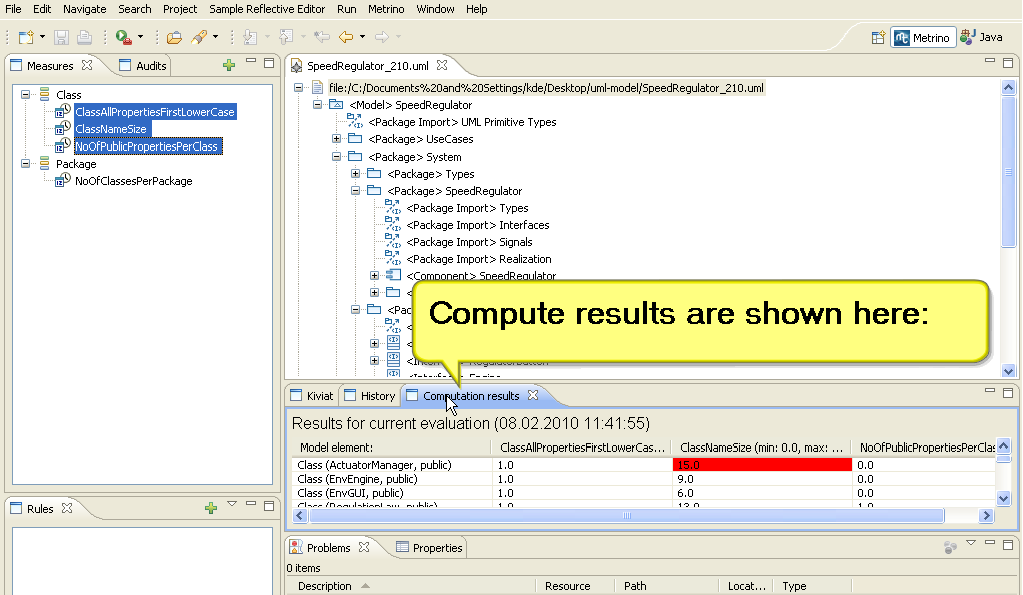
\includegraphics[width=\textwidth]{metrino_screen_1}
	\caption{Developement process and layers}
	\label{fig:sonarrunning}
\end{figure}

(generic validation by selected measures)

\begin{figure}[h]
	\centering
		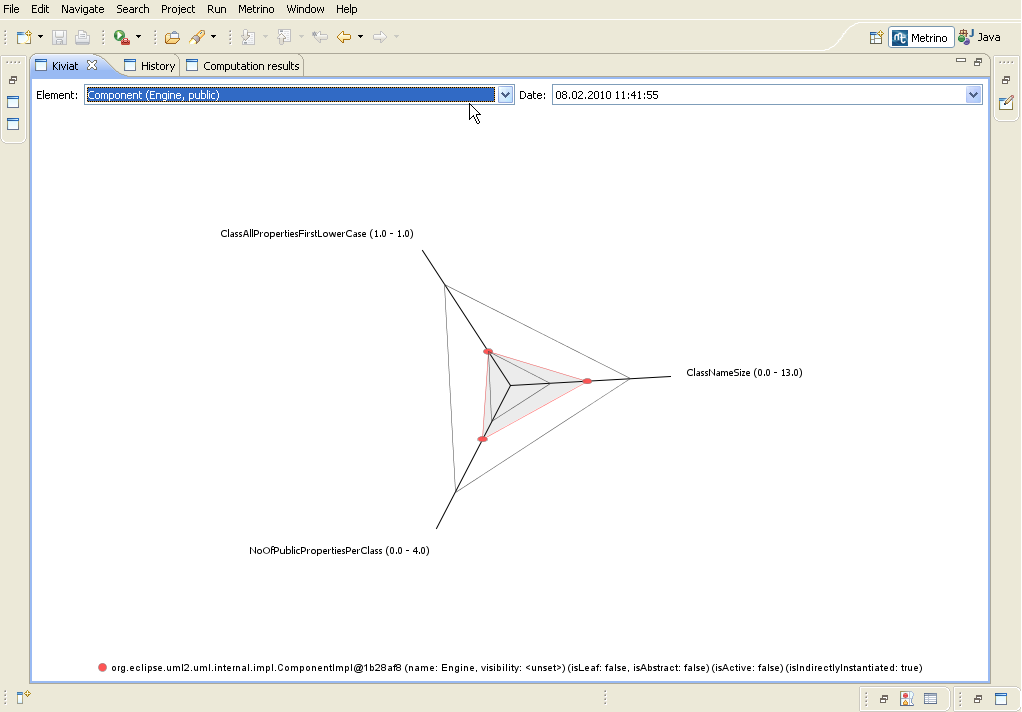
\includegraphics[width=\textwidth]{metrino_screen_2}
	\caption{Developement process and layers}
	\label{fig:sonarrunning}
\end{figure}

(graphical representation of a selected measurement)

\begin{figure}[h]
	\centering
		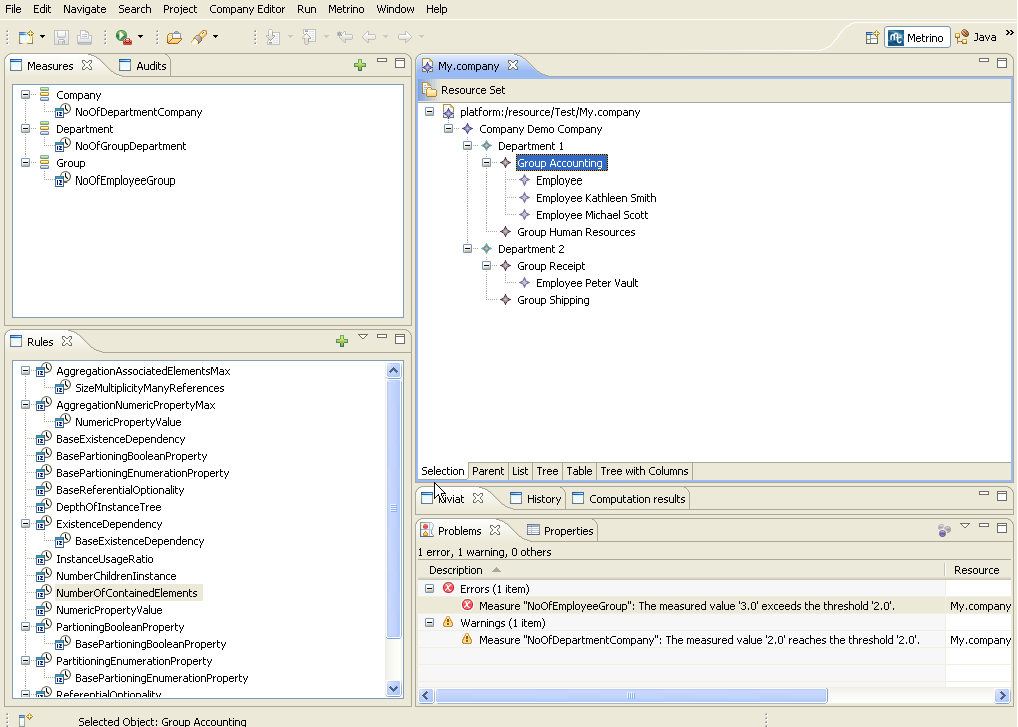
\includegraphics[width=\textwidth]{metrino_screen_3}
	\caption{Developement process and layers}
	\label{fig:sonarrunning}
\end{figure}

(rules, measures, problems and validation)

\subsection{Declaration of OCL rules}
With the models, we got from the Modelbus service we can start an analysis. Therefore we want to use Metrino, which expects OCL (Object Constraint Language) as a description of the requests. OCL generally spoken is a declarative language for describing rules which apply on UML-Models.

In OCL there are 7 constraints to distinguish: 1. Invariants have to apply on either an instance or an association. 2. Pre- and postconditions have to apply every time, when the according operation begins or ends. 3. Initial and derived values are the constraints for other derived values. 4. You can define new attributes and operations, that are not defined in the model. 5. If there is a state transition, guards have to apply.

With this set of rules, we can define metrics on the models.

\subsection{OCL}

\section{Sonar} \label{sec:sonar}

Sonar is an open platform to manage code quality. It offers reports on duplicated code, coding standards, unit tests, code coverage, complex code, potential bugs, comments and design and architecture.

Sonar consists of 3 components:

\begin{itemize}
\item A database that stores the configuration and results of quality analysis
\item A web server that is used to navigate the results of the analyzes and make configuration
\item A client that will run source code analyzers to compute data on projects
Covering new languages, adding rules engines, computing advanced metrics can be done through a powerful extension mechanism. More than 50 plugins are already available.
\end{itemize}

Primary supported language is Java. Other languages are supported with extensions. Several open source and commercial extensions can cover the following languages: C, C\#, PHP, Flex, Groovy, JavaScript, Python, PL/SQL, COBOL and Visual Basic 6.

It integrates with Maven, Ant and continuous integration tools (Atlassian Bamboo, Jenkins, Hudson).

\section{Developing Sonar Plugins}

\subsection{Building and Packaging}
To create a plugin for Sonar, at least Java 5 is needed. Maven is also required to compile and package the plugin. The documentation of Sonar says, that a recommanded way is to duplicate one of the example plugins, which can be found in the /plugins directory of the github repository: https://github.com/SonarSource/sonar-examples

It is recommanded to use /plugins/sonar-reference-plugin. The example plugin can be copied by cloning the repository. Github provides the possibility to download the repository directly.

The plugin can be built and deployed by executing in the plugin root directory, so for example /path/to/sonar-reference-plugin:

\begin{verbatim}
mvn clean install
\end{verbatim}

Thereafter a JAR file is generated in the /target directory. After copying this JAR to the /extensions/plugin directory of Sonar, the server has to be restarded. There you go, you packaged your own Sonar plugin.

\subsection{Creating an own plugin}
A Sonar plugin is a set of Java objects, which implement extension points, which are interfaces or abstract classes to model an aspect of the system and define contracts of what needs to be implemented. Such extensions could be pages in the web application or sensors generating measures.

This plugin extensions must be declared in a Java class, that extends org.sonar.api.Plugin. This class must then be declared in the pom with the property :

\begin{verbatim}
<artifactId>sonar-foo-plugin</artifactId>
<packaging>sonar-plugin</packaging>
<build>
    <plugins>
        <plugin>
            <groupId>org.codehaus.sonar</groupId>
            <artifactId>sonar-packaging-maven-plugin</artifactId>
            <version>1.1</version>
            <extensions>true</extensions>
            <configuration>
                <pluginClass>com.mycompany.sonar.MyPlugin</pluginClass>
            </configuration>
        </plugin>
    </plugins>
</build>
\end{verbatim}

There are also more advanced parameters like Maven descriptors, etc. possible. The full list of advanced parameters can be found here.

There is a list of all known sub-interfaces and implementing classes of org.sonar.api.Extension. The most important and well known extension points are listed here.

\subsection{Sensors and Decorators}
Two extension enable methods to save measures: sensors and decorators. In plugin development it is often a problem to decide which one to use.

\subsubsection{Sensor}

A sensor is invoked once during the analysis of the project. The sensor then can invoke a maven plugin, parse flat files or connect to web servers. The generated XML file is parsed and used to save the first-level of measures on resources (project, package or class). The sensor can access and save measures on the whole tree of resources. They generally are used to add measures at the lowest level of the resource tree.

\subsubsection{Decorator}

Decorators are used when all sensors have completed their work. The decorate method is called on every resource of a certain level bottom up. Decorators load (SELECT) and save (INSERT) measures. Because of contextual calls it is only possible to access the resource and its children. So decorators are generally used to consolidate measured at higher levels that have been added by sensors at lower levels.

\subsection{Modify the front-end of Sonar and working with sensors and decorators}
Our plugin front-end consists of the following structure:

\subsubsection{ModelbusMetrics.java}

Our class ModelsbusMetrics implements the Metrics Interface of Sonar. In this file we define all Metrics that we'll create in other files. The obligatory metric definitions consist of the name, key and the return type. Optionally you can add more parameters with the description, direction, setQualitativ, and setDomain methods. At least we have to define the method getMetrics() because of the interface Metrics. In this method we add all metrics to an array list and set this as return value of the getMetrics() method.

\subsubsection{ModelbusPlugin.java}

This file is the main entry point for Sonar. With annotations we can define some Plugin meta data like the description and the name. The class ModelbusPlugin extends the class SonarPlugin and has the method getExtensions(). We add in this method all Sonar extensions that we want to use like definition classes. batch classes or ui classes.

\subsubsection{ExampleSensor.java}

We created an exampleSensor to demonstrate how it must be defined. In this file it's possible to do all things you like to do. An example would be to connect to a server. In our case we don't need a sensor.

\subsubsection{RandomDecorator.java}

Our first decorator is a real random decorator. It will give a random value to all files.

\subsubsection{ExampleFooter.java}

It's possible to change the layout with plugins. This file implements the interface Footer. We just add the method getHtml() and return an example text to change the front-end layout of sonar.

\subsubsection{ExampleRubyWidget.java}

We can also add Widgets. The administrator can add widgets to the users layout. If our sensors get some values, the can be written from our widget and presented with plain text or with visual objects.

\section{Software Architecture}
The main architecture is described as the following. Our main software product is called the Sonar ModelBus Plugin which of course is a Sonar Plugin. This plugin, the project is dedicated to, implements a Metrino Adapter as well as a ModelBus Adapter. These sub programs are intended to communicate with the WebServices from Metrino and ModelBus.

\begin{figure}[h]
	\centering
		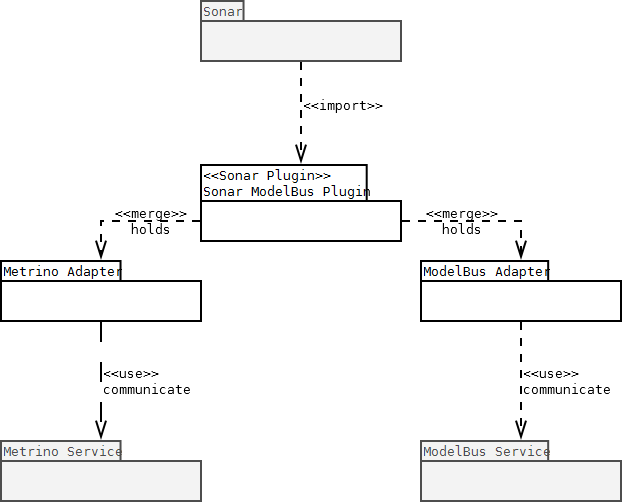
\includegraphics[width=\textwidth]{plugin_package_dia}
	\caption{Sonar plugin package diagram}
	\label{fig:sonarrunning}
\end{figure}

\begin{figure}[h]
	\centering
		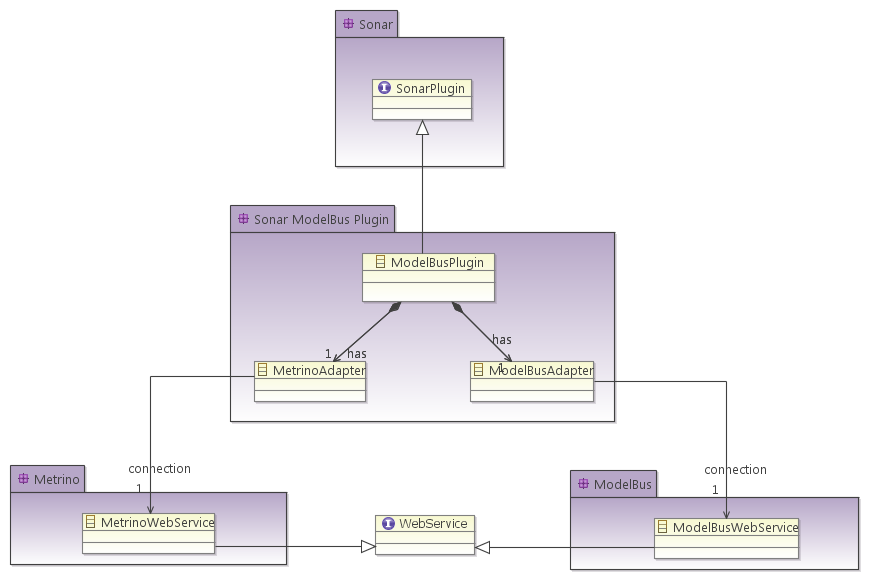
\includegraphics[width=\textwidth]{plugin_ecore_dia}
	\caption{Sonar plugin ecore diagram}
	\label{fig:sonarrunning}
\end{figure}


\section{Metrics Input File SMM}
SMM distinguishes between measures as the evaluation process of particular quality aspects of software artifacts and measurements which can be interpreted as the results of those processes. SMM specifies several types of measures and measurements for different outcome values:
\begin{itemize}
\item DimensionalMeasure
\item DirectMeasure
\item BinaryMeasure
\item CollectiveMeasure
\end{itemize}

The measures are calculated in a given scope, which has to be specified with \textit{scope="x"}, where \textit{x} is the id of a scope element, specified with \textit{xsi:type="SoftwareMetricsMetamodel2:Scope"}. Every measure also is part of a category, therefore it has to define its category with \textit{category="x"}, where \textit{x} is the id of a category element, specified with \textit{xsi:type="SoftwareMetricsMetamodel2:SMMCategory"}. This way measures can be categorized, so that one can measure different metrics in the same SMM file. Every category has an attribute measureElement, which simply holds the ids of the measures in the category. The results of the measures are saved in a measurement with \textit{xsi:type="SoftwareMetricsMetamodel2:DirectMeasurement"}. The id of this element has to be saved in the measurement attribut in the measure.

For more information, see Software Metrics Metamodel (SMM) on Wikipedia.



\section{Implementation}
\subsection{abc}










\section{Problems}

The following sections describe the problems we were confronted with during the development.

\subsection{Developing with Sonar}
The typical developement cycle with Sonar plugins is:
\begin{itemize}
	\item change the code of the plugin
	\item compile the plugin
	\item copy the compiled binary into the plugins folder of your Sonar server
	\item restart the Sonar server
	\item visit localhost:9000 and test your changes
\end{itemize}
This process can be automated with a special Maven goal. But the point is that the restarting of the server costs about 3-5 minutes!

%6. Entwicklung mit Sonar
	%	Dann insgesamt kann man die Dokumentation anmekern
		%zB Sonar
		%damit zu starten ist sehr einfach
	%%	aber sobald man was fortgeschrittenes machen will, muss man auf die Mailingliste

\subsection{Central repository}
In the beginning of the software project we tried to setup a central ModelBus server with Metrino service included for all team members. But it was not possible to run Metrino because it was only locally accessible and not over its remote URL. After compiling Metrino with remote settings the service did also not work. So we have chosen the other development way and installed ModelBus with Metrino on our local machines.
		
\subsection{Wrong class loader}
The problem was that we could not connect to the ModelBus repository through the sonar plugin. Using the same code in a standalone Java application instead worked fine: The ModelBus repository was successfully checked out.

The reason was that the ModelBus part could not resolve some bindings in its configuration. That was caused by the missing of a resource. This resource lied in the META-INF folder of the "org.modelbus.cxf.dosgi" jar bundle. The loading of this resource was done over the current context class loader in a ModelBus class:

\begin{verbatim}
ClassLoader cl = Thread.currentThread().getContextClassLoader();
Enumeration<URL> urls = cl.getResources("META-INF/cxf/bus/bus-extensions.txt");
//loading each url...
\end{verbatim}

The problem is that the context classloader of the current thread is not the plugin classloader.

Each Sonar plugin runs in an isolated classloader to avoid conflicts with other plugins. Third-party libraries can be loaded by using a mechanism specific to Sonar. It only requires to build the plugin with the sonar-packaging-maven-plugin, which copies the libs into META-INF/lib. This mechanism relies on its own classloader implementation.

By temporarly replacing the context class loader with the plugin class loader (the class loader of the extension), this issue can be solved:
\begin{verbatim}
ClassLoader initialClassLoader = Thread.currentThread().getContextClassLoader();
try {
  Thread.currentThread().setContextClassLoader(getClass().getClassLoader());
  //access ModelBus...
} finally {
  Thread.currentThread().setContextClassLoader(initialClassLoader);
}
\end{verbatim}

\subsection{Missing Metrino files}
Another problem was that the provided ModelBus copy was not complete concerning the Metrino service. Metrino was unable to compute the metric values for a given model. After copying the missing jar bundles (de.fraunhofer.fokus.metrino.ruleEvaluator and de.fraunhofer.fokus.metrino.measure) into ModelBus' plugins folder Metrino was ready for operation.

\subsection{No SMM standard}
To analyze a model for some metrics Metrino needs a SMM file, which defines the metrics with the help of OCL. The results of the model analysis will be saved in the SMM file again. So we needed to parse that SMM to retrieve the measurement results. The structure of the SMM file is defined by a XML schema. Unfortunatly, Metrino does not hew to the SMM standard. After browsing through the Metrino binaries we found the corresponding XML schema. Finally, we were able to parse the file and to retrieve the desired results.

\subsection{Displaying metrics per resource}
%2. Nichtanzeigen der Metriken pro Datei









\section{ModelBus Client Tool}
We created a tool for checking in and out files from/to the ModelBus repository. It can be simply called via "make":

Use
\begin{verbatim}
make checkin 
  URI=http://uri.de/location/in/repository/file.txt 
	FILENAME=location/to/local/file.txt
\end{verbatim}
to checkin a file located at FILENAME into the repository at a position defined by the URI.

Use
\begin{verbatim}
make checkout 
  URI=http://uri.de/location/in/repository/file.txt 
	FILENAME=location/to/local/file.txt
\end{verbatim}
to checkout a file from the repository located at URI to a local position defined by the FILENAME.
Changes can be made at the Client.java file. You can compile it by calling "make install". This will compile and assemble the client with its ModelBus dependencies.